%%%%%%%%%%%%%%%%%%%%%%%%%%%%%%%%%%%%%%%%%%%%%%%%%%%%%%%%%%%%%%%%%%%%%%%%%%%%%%%%
%2345678901234567890123456789012345678901234567890123456789012345678901234567890
%        1         2         3         4         5         6         7         8

\documentclass[letterpaper, 11 pt, conference]{ieeeconf}  % Comment this line out
                                                          % if you need a4paper
%\documentclass[a4paper, 10pt, conference]{ieeeconf}      % Use this line for a4
                                                          % paper

\IEEEoverridecommandlockouts                              % This command is only
                                                          % needed if you want to
                                                          % use the \thanks command
\overrideIEEEmargins
% See the \addtolength command later in the file to balance the column lengths
% on the last page of the document



% The following packages can be found on http:\\www.ctan.org
\usepackage{graphicx} % for pdf, bitmapped graphics files
\usepackage{graphics}
%\usepackage{epsfig} % for postscript graphics files
%\usepackage{mathptmx} % assumes new font selection scheme installed
%\usepackage{times} % assumes new font selection scheme installed
\usepackage{amsmath} % assumes amsmath package installed
\usepackage{amssymb}  % assumes amsmath package installed
\usepackage{hyperref}
\usepackage{bm}
\usepackage{algorithm2e}

\newcommand{\by}{\textbf{y}}
\newcommand{\bx}{\textbf{x}}
\newcommand{\bX}{\textbf{X}}
\newcommand{\bK}{\textbf{K}}
\newcommand{\cov}{\text{cov}}

\title{\LARGE \bf
Gaussian Processes for Crime Prediction
}

\author{Luis Perez$^{1}$ and Alex Wang$^{2}$% <-this % stops a space
\thanks{*A project for CS281, Fall 2015, Harvard University}% <-this % stops a space
\thanks{$^{1}$luisperez@college.harvard.edu}%
\thanks{$^{2}$alexwang@college.harvard.edu}%
}


\begin{document}

\maketitle
\thispagestyle{empty}
\pagestyle{empty}


%%%%%%%%%%%%%%%%%%%%%%%%%%%%%%%%%%%%%%%%%%%%%%%%%%%%%%%%%%%%%%%%%%%%%%%%%%%%%%%%
\begin{abstract}


The ability to predict crime is incredibly useful for police departments, city planners, and many other parties, but thus far current approaches have not made use of recent developments of machine learning techniques. In this paper, we present a novel approach to this task: Gaussian processes regression. Gaussian processes (GP) are a rich family of distributions that are able to learn functions. We train GPs on historic crime data to learn the underlying probability distribution of crime incidence to make predictions on future crime distributions.
\end{abstract}


%%%%%%%%%%%%%%%%%%%%%%%%%%%%%%%%%%%%%%%%%%%%%%%%%%%%%%%%%%%%%%%%%%%%%%%%%%%%%%%%
\section{INTRODUCTION}
The increased availability of open crime statistics has made it possible to use new machine learning techniques to aid in crime detection and prevention in order to help cities decide how to allocate scarce police resources. For example, foreknowledge on where a crime is likely to occur can tell police departments where and when additional officers could be stationed to preempt any crime. Detecting these crime-prone areas, also known as hotspots, has been a fixture of crime prevention. However, law enforcement agencies across the United States have only recently begun moving away from outdated analytic techniques (such as hot-spot identification \href{hotspot_mapping}) towards predictive approaches, such as hot-spot identification, regression, classification, and clustering models \cite{predictive_policing} \cite{hotspot_matrix}. Despite the increased interest in predictive analytics with large data demand and complexity, two problems remain: (1) conventional approaches remain prevalent due to their ease of use, and (2) more recent advancements in the ML community, such as neural networks and Gaussian processes, have not been explored with respect to this problem.

In this paper, we focus on tackling the second issue. In particular, we apply Gaussian processes (GP) to the task of predicting crime distribution in the selected cities of Boston and San Francisco. GPs are powerful non-parametric models that have proven effective in predicting other real-world, cyclical time-series data such as CO2 emissions and human motion \cite{gaussian_models}. In the following sections, we explore the the state of the art in terms of positive definite kernels \cite{kernel_methods}, and compare the resulting crime predictions with current baselines. We conclude with a discussion on the applicability of GPs to crime prediction, including their increasing accessibility, which combined with their power, demonstrates their usability in helping police departments and other interested individuals efficiently allocate resources.  
 
\section{MODEL}

\begin{figure}
\centering
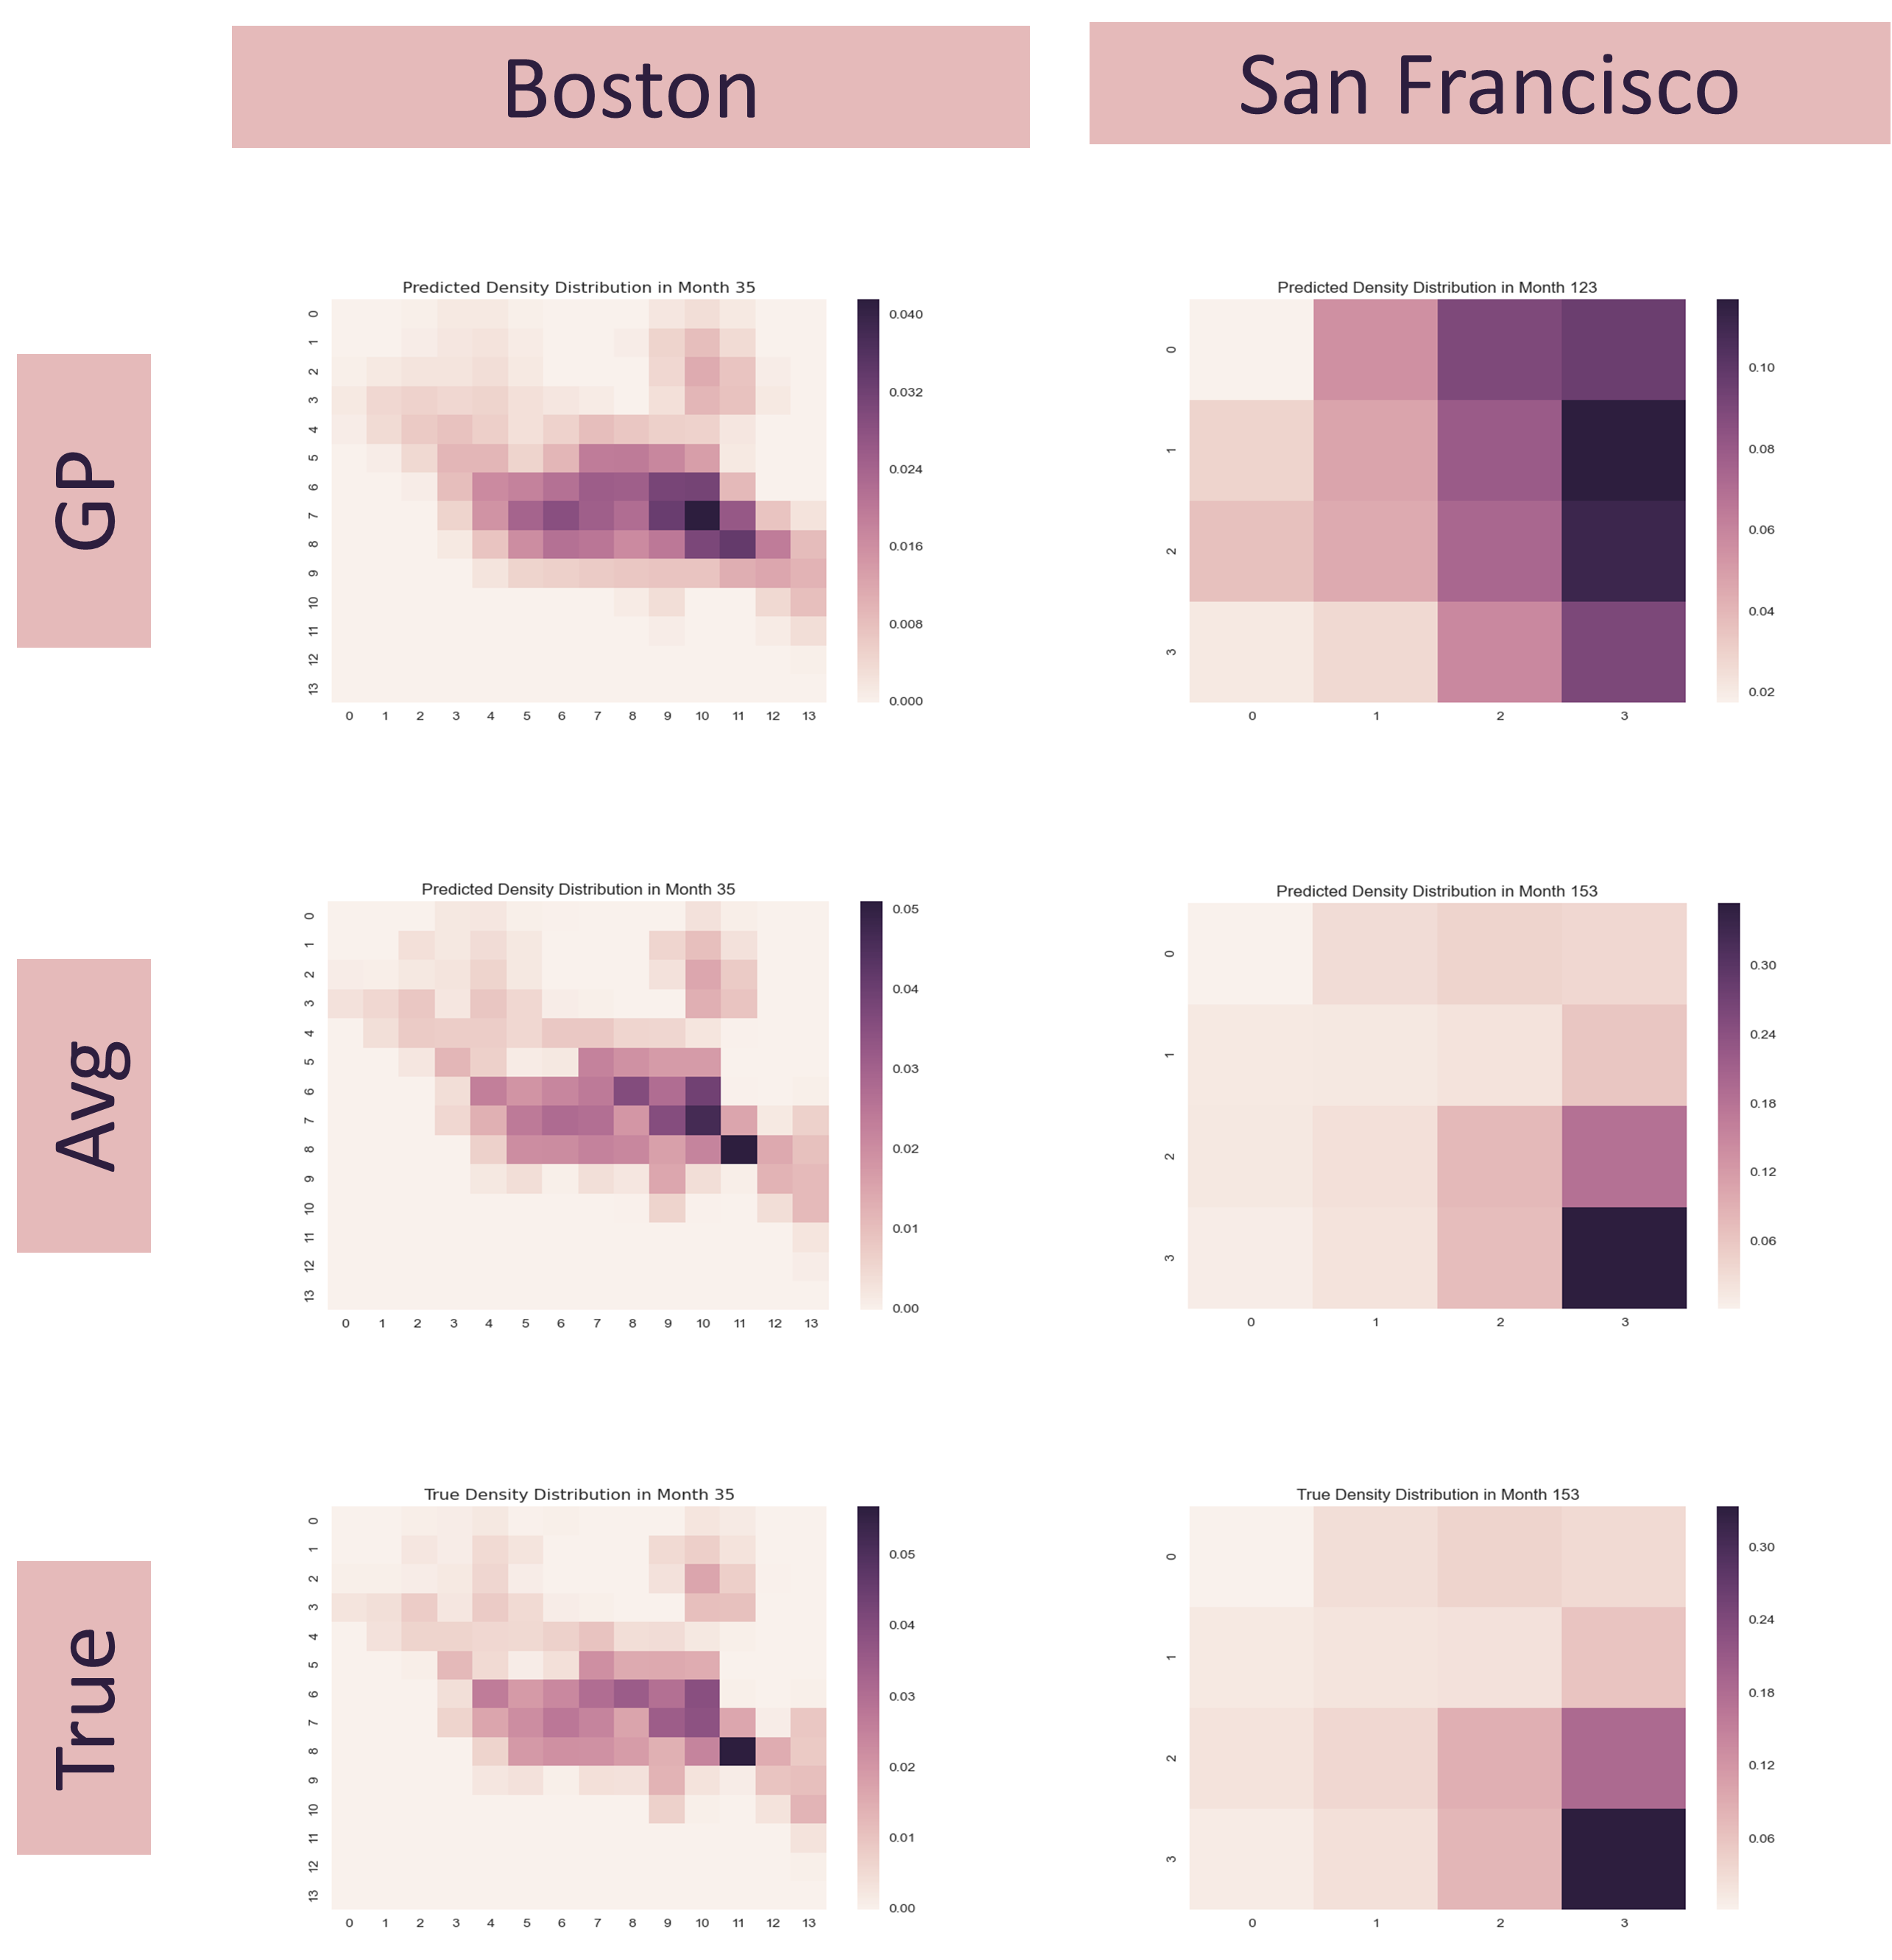
\includegraphics[scale=0.15]{heat_maps}
\caption{Distribution over the geography of tested cities with different models.}
\end{figure}
Formally, a Gaussian process is a collection of random variables, any finite number of which have a joint Gaussian distribution \cite{c1}. An intuitive interpretation of a GP arises when we think of it as a distribution over functions. GPs are a generalization of normal distributions to then infinite space of continuous functions (rather than continuous r.v.s). In this interpretations, any finite set of functions generated from a drawn function $f$ must be jointly distributed. Therefore, in training, we attempt to learn the underlying function space as seen in \ref{gm}. Continuing the analogy to a normal distribution, if a function $f(\bx)$ follows a GP distribution, then we write  
$$f(\bx) \sim GP(m(\bx), \kappa(\bx, \bx'))$$
where the GP is completely specified by a mean function $m(x)$ and positive definite covariance function $\kappa(\bx, \bx')$. Each are defined:
$$m(\bx) = \mathbb{E}[f(\bx)]$$
$$\kappa(x, x') = \mathbb{E}[(f(\bx) - m(\bx))(f(\bx') - m(\bx'))]$$

Following the definition of a GP, given a collection of points \bX, $f(\bX)$ follows a multivariate normal distribution:
$$p(\textbf{f}|\bX) = \mathcal{N}(\textbf{f}|\bm{\mu}, \bK)$$
$$K_{ij} = \kappa(\bx_i, \bx_j)$$
$$\mu = (m(\bx_1), \dots, m(\bx_N))$$

The most important hyper-parameter when working with Gaussian processes is the choice of the kernel function. The predictive performance of the GP is almost exclusively determined by this parameter. This is due to the fact that the kernel function determines if two points are ``similar'' in the input space to the drawn functions. It is this similarity between the points $x_i \sim x_j$ that force the output variables $f(x_i) \sim f(x_j)$ to be be close in value (with some added $\epsilon$ noise) \cite{c2}. Thus, the kernel function determines the range of possible shapes that the $GP$ will learn, and as we move further ``away'' from the input training data, impact more directly the predicted results.

One of the most common choice in literature, and one that has proven effective in many methods, is the squared exponential function \footnote{Also referred to as the the radial basis function (RBF)}. We present the multivariate form:
$$k_{\text{SE}}(\bx, \bx') = \sigma_f^2 \exp(-\frac{1}{2}(\bx - \bx')^\top \textbf{M} (\bx - \bx'))$$
where \textbf{M} is a diagonal matrix: $\textbf{M} = \text{diag}(\textbf{l}^{-2})$. The parameters are $\sigma_f^2$, the vertical scale of the function, and $\textbf{l}$, the horizontal scale with $l_d$ the scale factor for dimension $d$. A large scale factor for a dimension means that the feature is relatively less important. Often times we also assume that we have noisy output, so we add the noise term $\sigma_\epsilon^2 \delta_{\bx\bx'}$ with $\delta_{\bx\bx'} = 1$ if $\bx = \bx'$, $0$ otherwise.

Two other kernels worth mentioning because we make use of them in this paper are the periodic kernel:
$$k_{\text{per}}(\bx, \bx') = \sigma_f^2 \exp(-\frac{1}{2} \sum_d (\frac{\sin(\frac{\pi}{\lambda_d} (x_d - x'_d))}{l})^2$$
As the name suggests, the periodic kernel is periodic, and thus is useful for capturing cyclic patterns in data. The parameters $\sigma_f^2$ again controls the vertical and horizontal scales respectively, and serves a similar purpose of measuring the importance of each parameter as is the case with the exponential kernel. On the other hand, $\lambda_d$ controls the wavelength along dimension $d$, which relates to the frequency with which the kernel repeats itself \footnote{For a more detailed, yet accessible approach to kernels, we recommend the \href{http://people.seas.harvard.edu/~dduvenaud/cookbook/}{Kernel cookbook} by David Duvenaud}. 

We also have the linear kernel:
$$k_{\text{lin}}(\bx, \bx') = \sigma_b^2 + \sigma_f^2(\bx - \textbf{c})^\top(\bx' - \textbf{c})$$
The parameters $\sigma_b^2$ and $\sigma_v^2$ are the bias and scale term, similar to that of linear regression. In fact, if we were to simply use the linear kernel as our covariance function, we would actually be performing Bayesian linear regression \cite{c3}. The reason we include this kernel is that we can combine kernels via simple operations such as addition or multiplication and still have a valid kernel. Combining kernels in this way allows us to more accurately model different types of patterns.

   \begin{figure}[thpb]
      \centering
      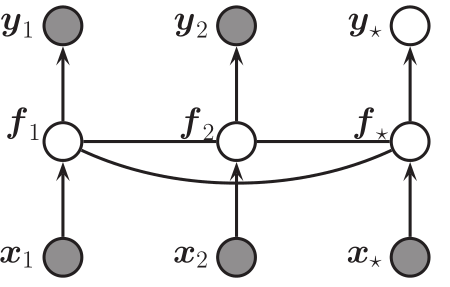
\includegraphics[scale=1.0]{graphical_model.PNG}
      %\framebox{\parbox{3in}{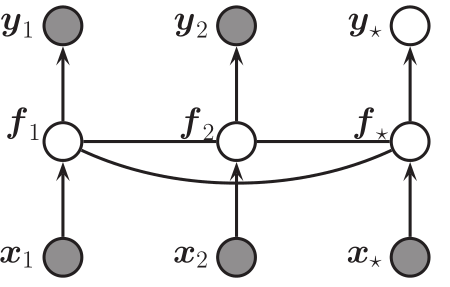
\includegraphics[scale=1.0]{graphical_model.PNG}}}
      \caption{Mixed graphical model for a noisy Gaussian process with two training points and one test point $\bx^*$. The function values $f_i = f(\bx_i)$ are all interconnected with edge weight $\kappa(\bx_i, \bx_j)$ while $y_i$ is the noisy output. We want to be able to predict $f(\bx^*)$. Figure borrowed from \cite{c2}}
      \label{gm}
   \end{figure}
Figure \ref{gm} shows the general graphical model for a Gaussian Process.

\section{INFERENCE}

We now describe how to make predictions with Gaussian process regression. We assume we have seen data points $\{\bx_i, y_i\}_{i=1}^N$ where $y_i$ is the noisy output of the underlying function $f$. In other words, $y_i = f(\bx_i) + \epsilon$ with $\epsilon \sim \mathcal{N}(0, \sigma_\epsilon^2)$. We denote $\bX = \{\bx_i\}_{i=1}^N$ and $\by = \{y_i\}_{i=1}^N$. We want to make predictions on a new set of inputs $\bX^* = \{\textbf{x}^*_i\}_{i=1}^M$. Equivalently, we want $f(\textbf{x}^*_i)$ for all $i$, the entire vector of which we denote $\textbf{f}^*$. 

From our model, we know that $\textbf{y}$ and $\textbf{f}^*$ are jointly Gaussian distributed:
$$\begin{pmatrix}
\by \\ \textbf{f}^*
\end{pmatrix} \sim \mathcal{N}\begin{pmatrix}
\textbf{0}, \begin{pmatrix}
\bK_y & \bK_* \\
\bK_*^\top & \bK_{**}
\end{pmatrix}
\end{pmatrix}
$$
where we assume that the mean of both is zero, $\bK_* = \cov(\by, \textbf{f}^*)$, and $\bK_{**} = \cov(\textbf{f}^*, \textbf{f}^*)$. Then we can use standard Gaussian conjugacy results to get the condition distribution of $\textbf{f}^*$:
$$p(\textbf{f}^*|\bX^*,\bX, \by) = \mathcal{N}(\textbf{f}^*|\bm{\mu}_*, \bm{\Sigma}_*)$$
$$\bm{\mu}_* = \bK_*^\top \bK_y^{-1} \by$$
$$\bm{\Sigma}_* = \bK_{**} - \bK_*^\top \bK_y^{-1} \bK_*$$
We take for our predictions the maximum a posteriori estimate, which for a Gaussian is the mean. Once the results are calculated, we convert them to a standard probability distribution by normalizing over the features space. 

One immediate complication is that it is not numerically stable to simply invert $\bK_y$ to compute the mean. Instead, we use a Cholesky decomposition, which we know exists because the kernel is positive definite. So, the final algorithm, which we take from Murphy \cite{c2}, is as follows
% \RestyleAlgo{boxed}
\RestyleAlgo{boxruled}
\LinesNumbered
\begin{algorithm}[ht]
  \caption{GP Regression\label{alg}}
  \textbf{L} = cholesky($\bK_y$) \\
  $\bm{\alpha} = \textbf{L}^\top \backslash (\textbf{L} \backslash \by))$ \\
  $\bm{\mu_*} = \bK_*^\top\bm{\alpha} $ \\
  $\log p(\by | \bX) = -\frac{1}{2}\by^\top \bm{\alpha} - \sum_i \log L_{ii} - \frac{N}{2}\log(2\pi)$
\end{algorithm}

Note that this algorithm is independent of the chosen kernel function. Therefore, we can abstract the kernel function so that we are free to explore different kernels \footnote{For more details, check our \href{https://github.com/kandluis/crime-prediction}{github}.}. 

\section{RELATED WORK}

Though the data-driven techniques for crime prediction have received increased research focus in recent years, there has been surprisingly little research on applying machine learning techniques to the task of crime prediction. The current cutting edge relies on older techniques, such as linear regression and clustering. Even current research in the field tends to approach the problem from a more analytic perspective, rather than a predictive model-focused approach. Traditionally, research has focused on either identifying hotspots of crime or clustering criminal activity by type of crime. Our paper falls in the former, and we proceed as such. 

The simplest approach to crime hotspotting, and indeed one used often in practice today \cite{c8}, is simply to analyze historical data and take historical high crime areas to be the high crime areas in the future \cite{predictive_policing}. We base our baseline model on this common method of crime prediction. The current state of the art in crime prediction is kernel density estimation (KDE), a technique similar to Gaussian processes. Some made-for-police software employs this technique \cite{predictive_policing}, and it is still prevalent in research, as Gerber \cite{c7} used it with Twitter data to predict crime. To our knowledge, complex machine learning models such as Gaussian processes, neural networks, etc. have not been applied to this domain. Even those techniques that have found some success are nonetheless not typically applied due to their difficulty or un-interpret-ability. In this paper, while we focus on exposition of a novel technique, we make an effort to make our results and software accessible to other researchers in the hope of creating guiding the production of an intuitive system.

However, shifting focus back to the research presented, we note that most attention has gone towards identifying spatial patterns in crime data, such as geographic distribution of crime. Extension appear limited to more complex categorization of the crime by type, weapon used, etc. Temporal patterns in the data receive far less attention \cite{hotspot_matrix}, though it is common knowledge that crime tends to be cyclic. In this sense, the aforementioned approaches are limited in that they do not seek to incorporate temporal patterns or changes. There have been some attempts to consider temporal features such as time of day or season \cite{predictive_policing}, but to our knowledge there is no comprehensive model that takes into account spatial features as well as larger macro trends to be found in spatial data.

Gaussian processes have been quite widely studied \cite{c1} and have been used for a variety of regression tasks, ranging from real-time tracking \cite{c9} to water resource usage \cite{c10}. In general their application to time-series is not a new; their ability to predict time-series data relatively well is known. In fact, we find it surprising that these models have not been applied to the seemingly simple task of predicting crime data, and therefore maintain a very simplistic approach in our model to avoid over-complicating the research. 

\section{EXPERIMENTAL SETUP}

\subsection{Dataset}

We use public city crime datasets from Boston and San Francisco. These datasets document reported crimes that occur from 2012-2015 and 2003-2015 respectively. The datasets contained $253075$ and $1834080$ entries respectively. We also performed preliminary exploration on a the crime data set from Chicago, though the size of the data proved restrictive with our limited computational resources. Each dataset contains information on the type of crime, the time and date of the crime, geographic information including ward and latitude/longitude, etc. 

For our experiments, we extracted the latitude and longitude of the crime, and the date of the crime. We created $n$ buckets for each of latitude and longitude, for a total of $n^2$ buckets, where $n$ is an additional hyper-parameter to tune. We attempted tuning of this hyper-parameter using standard techniques such a gradient ascent on the log-likelihood. However, we found no optimal parameter, with the log-likelihood increasing for the tested values of $n$, which ranged from $n = 1$ to $n = 25$ on the Boston data set and $n = 2$ to $n = 15$ on the San Francisco data. We also convert the date to months since first month in the dataset. Lastly, once the data has been partitioned for a fixed $n$ value, we count the number of crimes in each region as specified by the Latitude and Longitude. We also clean the data of outliers, in particular, we remove the last month of the crime data from each data set as each is incomplete. We found no other immediately discrepancies in the data, even after thorough preliminary analysis  

Testing data consists of two methods: (1) holding out the last year of crime data and (2) randomly splitting into $80\%$ training data and $20\%$ testing. We found method (1) to be the most informative and also the most effective, and therefore trained all of our models under this method. Method (2) was used for training only for the baseline and the standard exponential kernel. Due to computational limitations, we refrained from continuing the use of method (2).

All data in the obtained data sets was ignored except for the three features mentioned above. We expect that incorporating more of this data, while increasing the computational complexity of training our model, will prove extremely useful.

\subsection{Baselines}

Our baseline for future months is historical average crime count per bucket. This is an approach still employed today, mainly because it has proven effective. We then normalize the count in each bucket by the total in order to get a probability distribution.

To compare our method against the baseline, we compute the Kullback-Leibler (KL) divergence of both the baseline distribution and the GP distribution with the true distribution for the most recent year. That is, we compute:
$$KL(p||q) = \sum_i p(i) \log \frac{p(i)}{q(i)}$$
KL divergence gives a measure of the cost of modeling distribution $p$ with distribution $q$, so a lower KL divergence is better. Furthermore, $KL$ divergence is interpret-able as measuring the  Multiple interpretations of $KL$ divergence exists, but among the best, we have (1) $KL$ divergence as a measure of information gained when we move from the distribution $q$ to the distribution $p$ (from the distribution our model computes to that computed observed). In this sense, the $KL$ divergence measures the amount of information lost through our model as opposed to actually waiting to observe the data. A second interpretation, which might be more intuitive to computer scientists, is that of $KL$ divergence measuring the expected number of extra bits required to encode samples from $p$ using a code optimized for $q$ rather than the code optimized for $p$. The latter interpretations is the most suitable for our model.

\subsection{Implementation}

We implemented Gaussian process regression ourselves as well as two kernels, the squared exponential kernel and a periodic kernel. To verify the correctness of our code, we compare the computed likelihood of our model against that of the GPy library for the same kernel and inputs (\url{https://github.com/SheffieldML/GPy}). After verifying correctness, we use our own kernels for future computations, with the exception of computations found to be too expensive (such as training over a large parameter space). In such scenarios, we make use of the GPy framework to calculate results presented in this paper. 

Newt, we fix the noise variance to be the standard deviation of the training data, then attempt to tune the parameters by maximizing log likelihood (as computed via \ref{alg}). While this fixed value was picked based on intuition, we have consider some other alternatives. For example, we can make use of the law of total variance to calculate the appropriate noise values as given our data $D$ to be:
$$
E[\text{Var}(X \mid D)] = \text{Var}(X) - \text{Var}[E(X \mid D)]
$$
Further exploration into this idea is useful, though we defer such exploration to future research. 

We use the scipy implementation of L-BFGS for a max of 150 iterations, or less if the optimization procedure converges beforehand, in order to optimize our kernel parameters. All parameters for all kernels are initialized to the default values if using the GPy library, otherwise all parameters are initialized to a default value of$1$. The kernel's are then optimized using the log-likelihood as the output function. We do not expect over-fitting to occur, especially given the statistical nature of GPs.  

Once we have the tuned model, we generate predictions for the amount of crime in each bucket for the most recent year (or the random points, if that was the hold-out data). The predictions tended to be in par most of the time, though we did find that some of the results appeared somewhat intuitive. 

For example, most of the he models predicted positive values, but some times a model would try to predict slightly negative values. In such a scenario, the values were clipped to be some $\epsilon > 0$. Then, we normalize by the total crime across the entire test set to get a probability distribution of crime for the most recent year. This way, we are able to not only get relative probabilities of crime across geography, but over time as well. 

We also decided to explore combinations of kernels, for which we used the GPy library. Using \cite{c3} as guide, we decided to fit the following kernels: linear * periodic and squared exponential * periodic. The reason for this choice of kernels is obvious. We wish to incorporate some fixed periodicity into our data. We propose that yet another kernel available for exploration is the locally periodic kernel, which might prove sufficient on its own at tackling the task of correctly interpolating the crime data points. 

For each composite kernel, we use the same optimization process as described above. We also calculate the marginal likelihood and the $KL$ divergence using the predictive methods already described. 

\section{RESULTS}

Our main results are presented in Tables 1 and 2 for Boston and San Francisco respectively, presenting our main quantitative findings. We also include Figures \ref{fig:log_likelihood}, \ref{fig:baseline_results} and \ref{fig:predictive_results_boston} for reference in the discussion, as they provide a qualitative interpretations to our data.

\begin{figure}
\centering
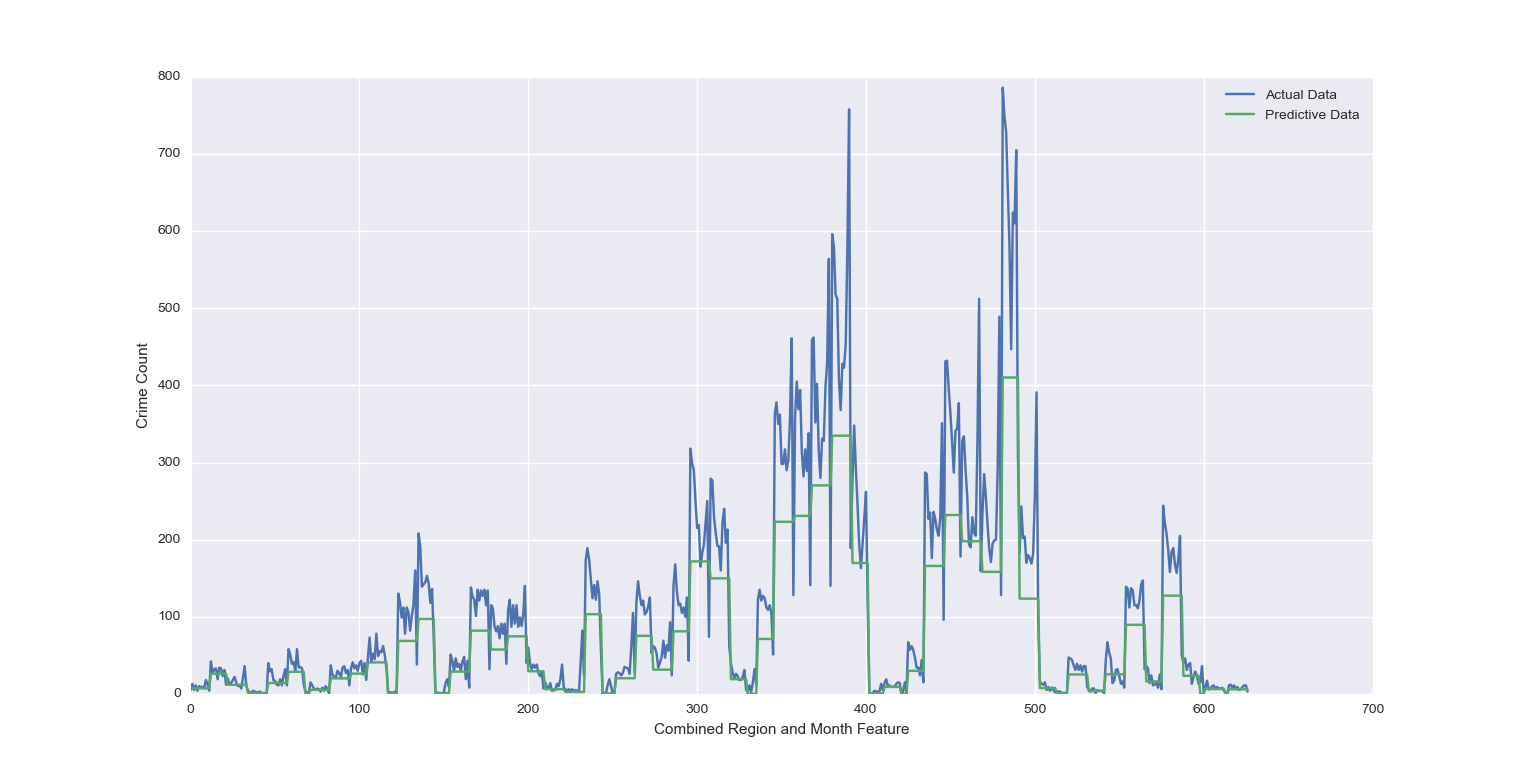
\includegraphics[scale=0.11]{baselines_count}
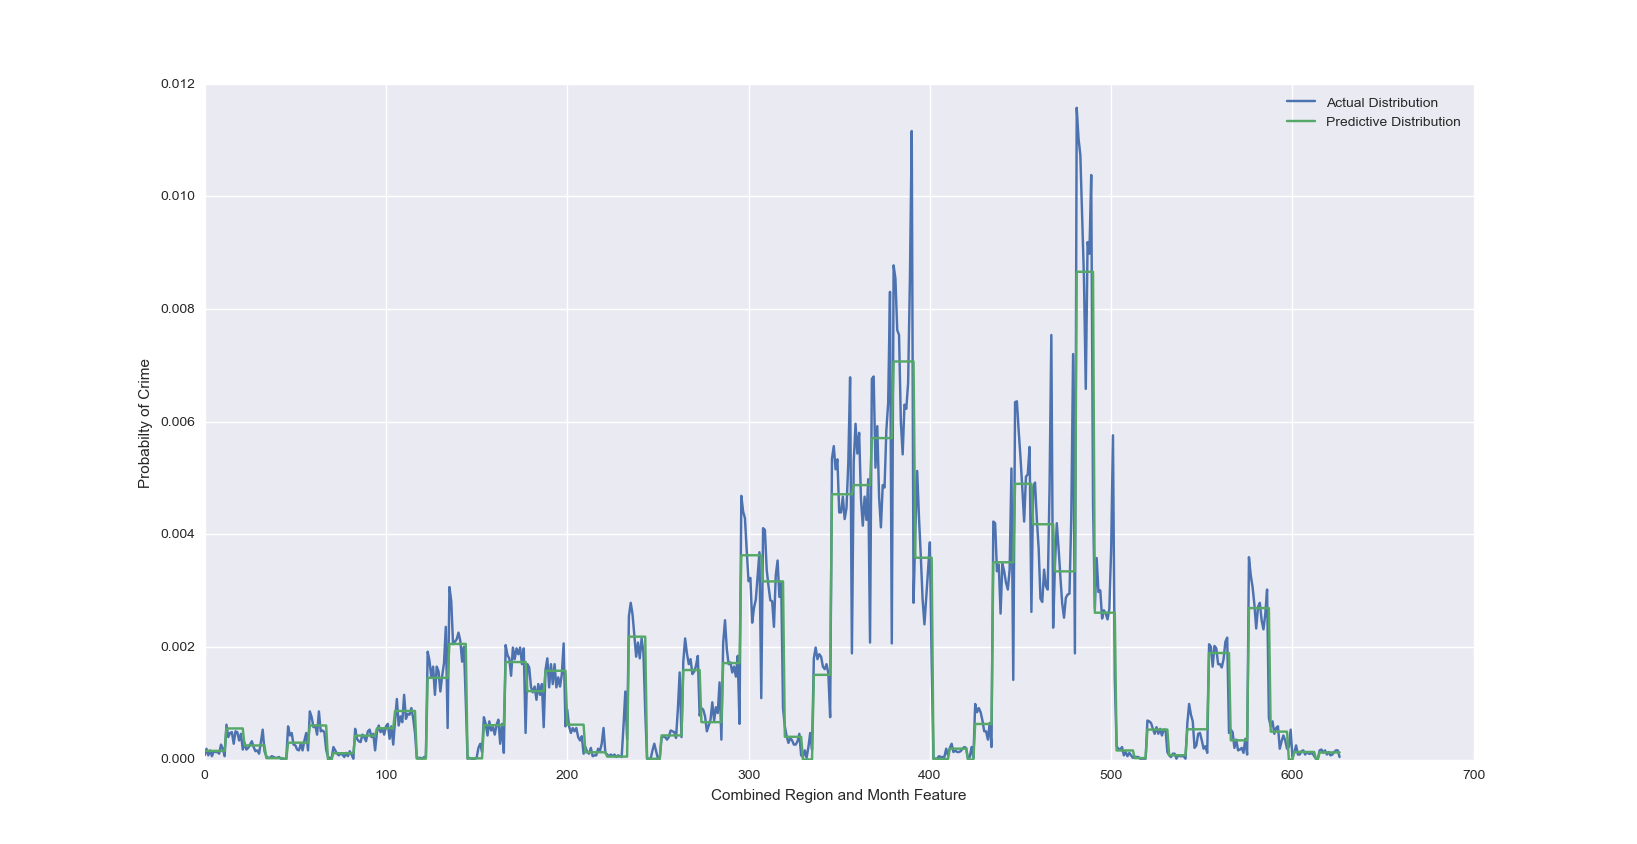
\includegraphics[scale=0.11]{baselines_distribution}
\caption{The crime count (top) and crime distribution (bottom) over our entire sample set using the results of our baseline model. Note that the baseline model tends to over-predict as we move further away from our training data, temporally.} 
\label{fig:baseline_results}
\end{figure}
Figures \ref{fig:baseline_results} show the predicted distribution overlaid with the test data distribution. The average appears to be quite adequate at predicting crime in the future, especially when it comes to geographical predictions. However, it has many theoretical limitations as it will not be able to learn from previous cyclic patterns, and in particular, it is unable to learn that crime has a general decreasing trend. 

\begin{figure}
\centering
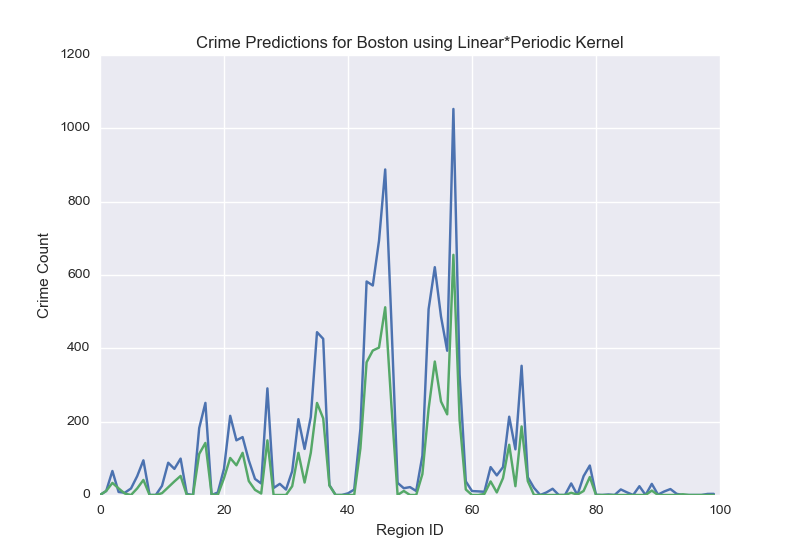
\includegraphics[scale=0.2]{predicted_lin_per_count}
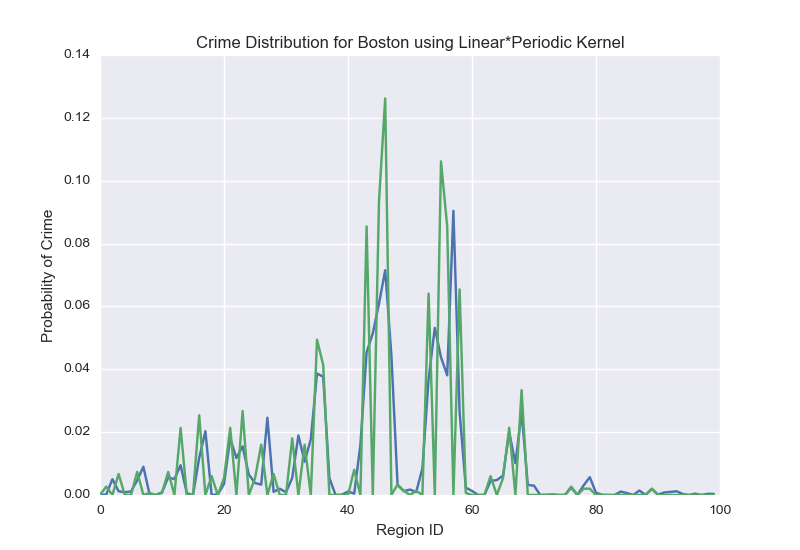
\includegraphics[scale=0.2]{predicted_dist_lin_per_count}
\caption{(Left) Crime count predictions using a combination of linear-times-periodic kernel. The results are promising, though we still run into the issue of under-fitting the crime predictions. The predictions are for the month immediately following our training data. (Right) We presented the normalized distribution of crime over the regions for the final month in our testing set. The distribution is for the final month in our testing data. The plot is a clear demonstration of the predictive power of GPs.}
\label{fig:predictive_results_boston}
\end{figure}

We first explored the hyper-parameter $n$ to attempt to find an optimal bucketization of our regions. We discovered that such a problem appears to be somewhat ill-defined, and the results provided little insight. More computational resources are required in order to verify the existence of an optimal, though we hypothesized that the log-likelihood will continue to increase as the hyper-parameter $n$ increases. See Figure \ref{fig:log_likelihood} for a sample graph of the results. KL divergence was too found to be insufficient in this regard (See Figure \ref{fig:kl_divergence}), as it too increases without bound. We settled on picking a value which matched the computational resources available to us. 

\begin{figure}
\centering
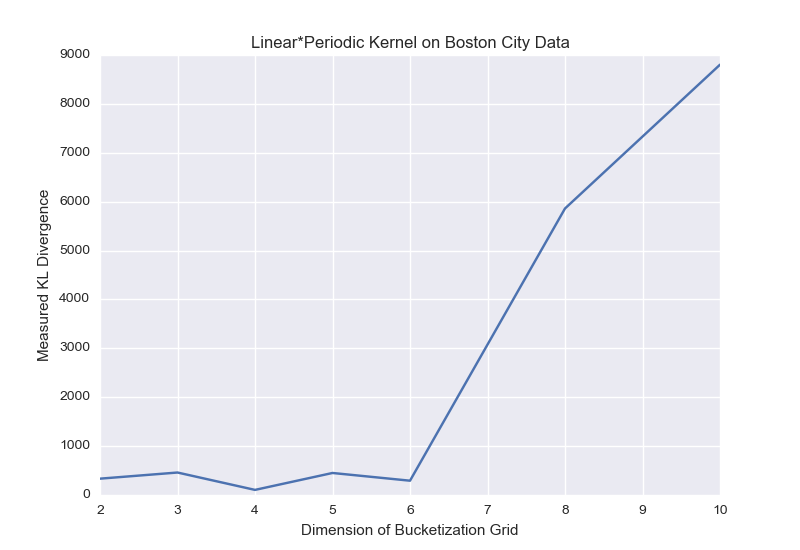
\includegraphics[scale=0.4]{kl_periodic_linear_periodic}
\caption{KL Divergence plotted against bucket size. The calculations are done on the Boston data set and occurs with optimized linear*periodic kernels. The optimization is done using standard maximization techniques.}
\label{fig:kl_divergence}
\end{figure}

We expected the composite kernels to perform best as they would be able to capture not only the temporal cycles in crime behavior, but also the larger macro trend of decreasing amount of crime. Interestingly, however, the linear-periodic kernel had mixed results. In Boston, it achieved the lowest KL divergence but the highest likelihood, both by significant margins. In San Francisco, it had the lowest likelihood but the highest KL divergence. We speculate that one reason for this is that the composite kernels have more parameters. For a periodic kernel alone, there are two parameters, wavelength and scale, for each dimension. Combining with a squared exponential or linear kernel adds to the number of parameters to be tuned. With additional optimization, we think the composite kernels would be able to perform better than the simpler kernels. In particular, we've begun exploration of the input parameter space through the use of Spearmint, a Bayesian Optmization framework based on GPs \cite{bayes_opt}. Results are currently preliminary, and the results presented in the paper make use of more typical techniques such as gradient descent/ascent and LBFG-S.

\begin{figure}
\centering
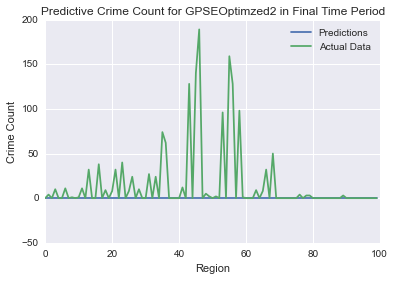
\includegraphics[scale=0.2]{Optimized_Final_Period_Crime_Count}
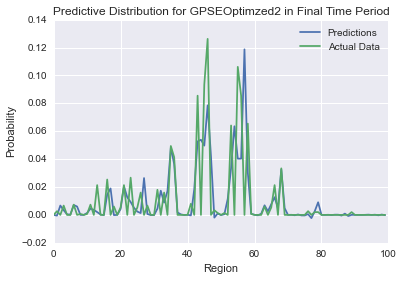
\includegraphics[scale=0.2]{Optimized_Final_Period_Distribution}
\caption{Crime Count and distribution for the optimized standard exponential kernel.}
\label{fig:final_period}
\end{figure}
A particular point of interest was the inability for the normal square exponential kernel to predict precise crime counts in far out into the future. As we can see from Figure \ref{fig:final_period}, the standard exponential kernel decreases rapidly temporally after the first few months. We believe this either to be a (1) limitation of the model itself, as we assign as $0$ mean function prior or (2) an after-effect of over-optimization which might have led to over-training on the spatial parameters rather than the time-parameter. The second explanation appears reasonable as it accounts for the fact that the model did not perform well . Despite the above limitations however, the model appears to predict the distribution of crime still relatively well. 

Another salient point is the significant differences in order of magnitude between the scores of Boston and San Francisco, especially for KL divergence which is two orders of magnitude less for San Francisco. We attribute this to the smaller bucket size we were resource-constrained to choose for San Francisco ($n=5$ vs $n=10$ for Boston). Because of this, the distribution for San Francisco was smoother than that of Boston, and thus easier to fit. Furthermore, in general we believe that KL is increasing in $n$ as we are trying to fit more probabilities, and thus adding more terms to the sum (of KL divergence for a discrete distribution). Therefore, we do not use KL divergence to compare Gaussian processes for different $n$. Instead we use likelihood, which we present in Figure \ref{fig:log_likelihood}. 

\begin{figure}[h!]
\centering
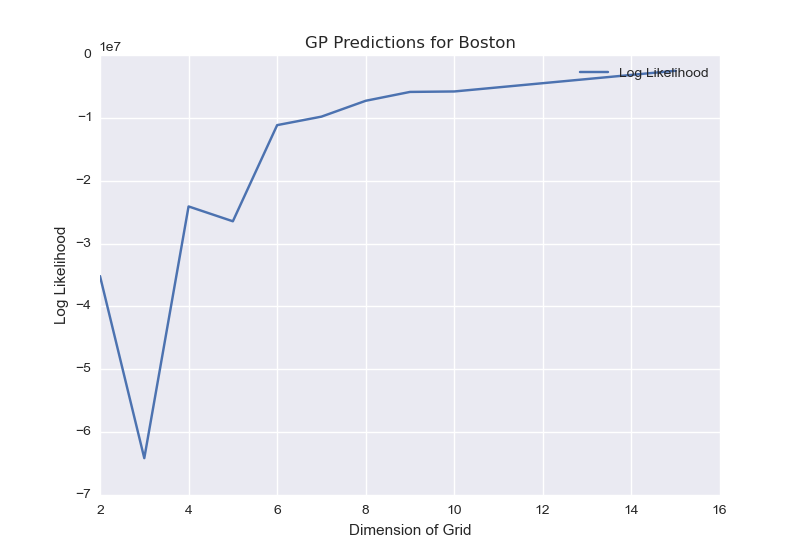
\includegraphics[scale=0.2]{GPSE_log_likelihood}
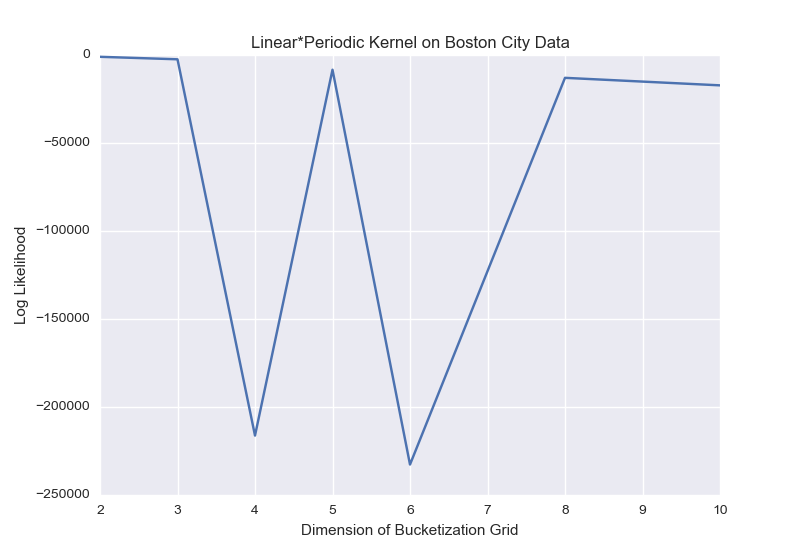
\includegraphics[scale=0.2]{kl_likelihood_periodic_linear_periodic}
\caption{Log likelihood vs bucket size, using the standard exponential kernel (left) and a linear*periodic kernel (right) on the Boston data set. It is indeterminate as to what to expect for other kernels. Theoretically, the $n$ is regularized in the likelihood term ($-\frac{N}{2}\log(2\pi)$), so we expect the likelihood to fall off beyond a certain $n$, but due to computational restrictions, we weren't able to find that point.}
\label{fig:log_likelihood}
\end{figure}

We now consider the order of magnitude of our results. We were unable to find any papers that present results in terms of the KL divergence when considering Gaussian processes. However, intuitively, we interpret the results to be inconsistent. The baselines for both cities are orders of magnitudes below the results obtained though GPs. We believe the reason for this discrepancies has to do with our already low probability distributions over the region. Any small mismatch can lead to large $\frac{p(x)}{q(x)}$ values which can cause the $\log$ function to increased rapidly. However, as with any software project, despite our best efforts it is entirely possible that there exists some sort of bug in our code that leads to the values presented. Despite this, we're relatively certain that the results are not invalid, and instead opt for a second explanation. $KL$ divergence appears to the ill-suited for our task. The predictive distributions plotted both as heat-maps and line-graphs appears to math the test distribution extremely well.   

\begin{table}[h]
\caption{Boston Results for Various Methods ($n=10$)}
\label{table_bos}
\begin{center}
\begin{tabular}{|c|c|c|}
\hline
Method & KL Divergences & Likelihood\\
\hline
Baseline & 0.138 & NA \\
Sq Exp & 16264.067 & -17409.365 \\
Periodic & 13922.491 & -17801.469 \\
Lin*Per & 10979.432 & -24808.536 \\
SE*Per & 14265.814 & -17204.823 \\
\hline
\end{tabular}
\end{center}
\end{table}


\begin{table}[h]
\caption{San Francisco Results for Various Methods ($n=5$)}
\label{table_sf}
\begin{center}
\begin{tabular}{|c|c|c|}
\hline
Method & KL Divergences & Likelihood\\
\hline
Baseline & 0.436 & NA \\
Sq Exp & 632.411 & -30978.876 \\
Periodic & 631.510 & -30192.276 \\
Lin*Per & 923.175 & -29498.413 \\
SE*Per & 648.268 & -32984.243 \\
\hline
\end{tabular}
\end{center}
\end{table}


\section{FUTURE WORK}
The paper explored the intersection between practical crime prediction and novel ML techniques for time series prediction. Results show some promise, though we propose a more thorough discussion of the topic of accurately gauging the predictive power of our models. 

As referenced throughout the paper, we now focus on some possible extensions to our work. The first and simplest involves simply generalizing our methods to larger data sets. It would be of interest to see what effects this would have on a Gaussian process. In particular, we recommend extending the work to the Chicago dataset which will require significantly increasing the available computational resources or exploring sparse GP methods.

A second extension to our work is two-fold: (1) exploring further combinations of kernels, and (2) optimizing the parameters of the currently explored kernels further. This second extension is a natural continuation of the first. While both parts of the extension are of importance, we recommend the second. Parameter optimization has shown to be effective \cite{bayes_opt}, and we expect such results would also prove true here. Furthermore, Bayesian optimization is particularly promising for GP models and for data sets of similar size of our own.

Additionally, we maintained a rather simple model. We seek to predict crime at a particular location and time, and therefore used only three parameters for inputs (latitude, longitude, month). However, we expect that including and correctly incorporation additional data into the model will prove beneficial to our ability to predict crime. Most importantly, the Gaussian process framework we have presented in this paper is easily generalization to include more features. The domain of the function $f: \mathbb{Z}^3 \to \mathbb{R}^+$ is easily extensible to incorporate additional parameters. We expect such additional data will increase the need for computational resources. 

To address the final issue directly, future work in this area could focus in exploring sparse Gaussian processes. At at introductory level, sparse Gaussian processes find a smaller number of pseudo-data points to get a fair approximation of the GP while being more tractable as the size of the training data increases. 

Another area of improvement is log-Gaussian Cox processes, which would constrain positive predictions without need for clipping or converting to log-space. We suspect that a reason for our extreme KL divergence values is the necessity of adding $\epsilon$ for numerical stability, which caused extreme values in the sum of the KL divergence. An alternative approach to this positive constraint might lead to better metrics to compare against baselines.

We expect all of the above explorations to prove fruitful.
   
\section{CONCLUSION}

In this paper we presented a novel approach to crime prediction that makes use of Gaussian processes. Despite the fact that our proposed metrics for validation, such as log-likelihood, RMSE, and KL-divergence have shown to be somewhat ineffective at capturing the predictive ability of our system, we believe GPs to be a tool worth exploring further. With improved objective measures of predictability, such as teasing out the effectiveness in learning the proposed dimensions, we expect future research to prove significantly more fruitful, as our more qualitative measure of performance show significant advantages over baseline.

\begin{figure}
\centering
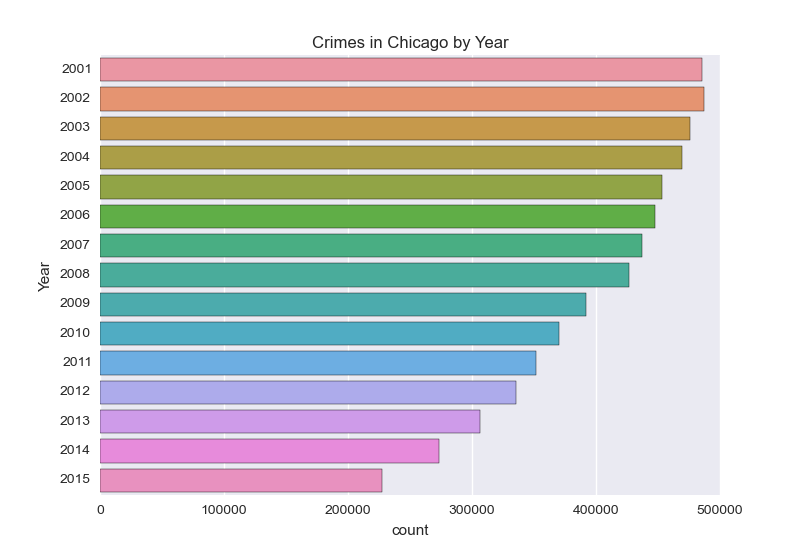
\includegraphics[scale=0.4]{chicago_crimes_by_year}
\caption{Early exploration of the Chicago data set shows promising patterns. While most cities across the united states have been extremely effective at reducing overall crime rates, Chicago's decline is the most pronounced. We expect such a problem for pattern discovery to be well-suited as a testing framework for the predictive power of GPs. }
\label{fig:chicago_data}
\end{figure}

This paper only serves as exploratory step into applying advanced machine learning techniques to the problem of crime prediction. There still remains much work to be done and a lot of promising areas to pursue: modern sparse kernels, new data sets, feature transformations, etc. 

While the results we present have only been shown to have adequate predictive power for the cities of Boston and San Francisco, we expect such methods to generalize well to other cities. In particular, we recommend their application to the city of Chicago, which as shown in Figure \ref{fig:chicago_data} has the potential for posing unique challenges by pushing the predictive ability of GPs. With further research, we believe GPs are good candidates for incorporation into the current system of crime prediction and analysis in place thorough major cities in the United State. 

It is our sincere hope that this paper will spur further investigation into applying current ML methods to practical problems facing our country today. 

All code can be found at \url{https://github.com/kandluis/crime-prediction}, and the specific data used can be accessed upon request. 

\addtolength{\textheight}{-12cm}   % This command serves to balance the column lengths
                                  % on the last page of the document manually. It shortens
                                  % the textheight of the last page by a suitable amount.
                                  % This command does not take effect until the next page
                                  % so it should come on the page before the last. Make
                                  % sure that you do not shorten the textheight too much.

%%%%%%%%%%%%%%%%%%%%%%%%%%%%%%%%%%%%%%%%%%%%%%%%%%%%%%%%%%%%%%%%%%%%%%%%%%%%%%%%



%%%%%%%%%%%%%%%%%%%%%%%%%%%%%%%%%%%%%%%%%%%%%%%%%%%%%%%%%%%%%%%%%%%%%%%%%%%%%%%%



%%%%%%%%%%%%%%%%%%%%%%%%%%%%%%%%%%%%%%%%%%%%%%%%%%%%%%%%%%%%%%%%%%%%%%%%%%%%%%%%

\section*{ACKNOWLEDGMENT}

We would like to thank the CS281 staff for putting on a great course. In particular we would like to thank Professor Doshi-Velez and David Duvenaud, both of whom gave us excellent advice at numerous points on how to proceed. Furthermore, we would like to thank the students in the class who contributed to our ideas through their honest discussion.


%%%%%%%%%%%%%%%%%%%%%%%%%%%%%%%%%%%%%%%%%%%%%%%%%%%%%%%%%%%%%%%%%%%%%%%%%%%%%%%%


\bibliography{references}
\bibliographystyle{plain}

\end{document}
